% =============================================================================
% KIẾN TRÚC HỆ THỐNG
% =============================================================================

\section{Kiến trúc hệ thống}
\label{sec:architecture}

Phần này mô tả kiến trúc tổng quan của hệ thống Crypto Analytics Platform dựa trên \textbf{Version 4: Microservices Event-Driven}---kiến trúc hiện đang được triển khai trong dự án.

\subsection{Sơ đồ kiến trúc tổng quan}

Hình~\ref{fig:arch-v4-overview} minh họa các thành phần chính của hệ thống và mối quan hệ giữa chúng. Luồng dữ liệu chính: Client gửi request qua API Gateway (Traefik); Gateway định tuyến đến các microservice tương ứng; các service giao tiếp bất đồng bộ qua Kafka và truy cập dữ liệu qua PostgreSQL/Redis.

\begin{figure}[H]
\centering
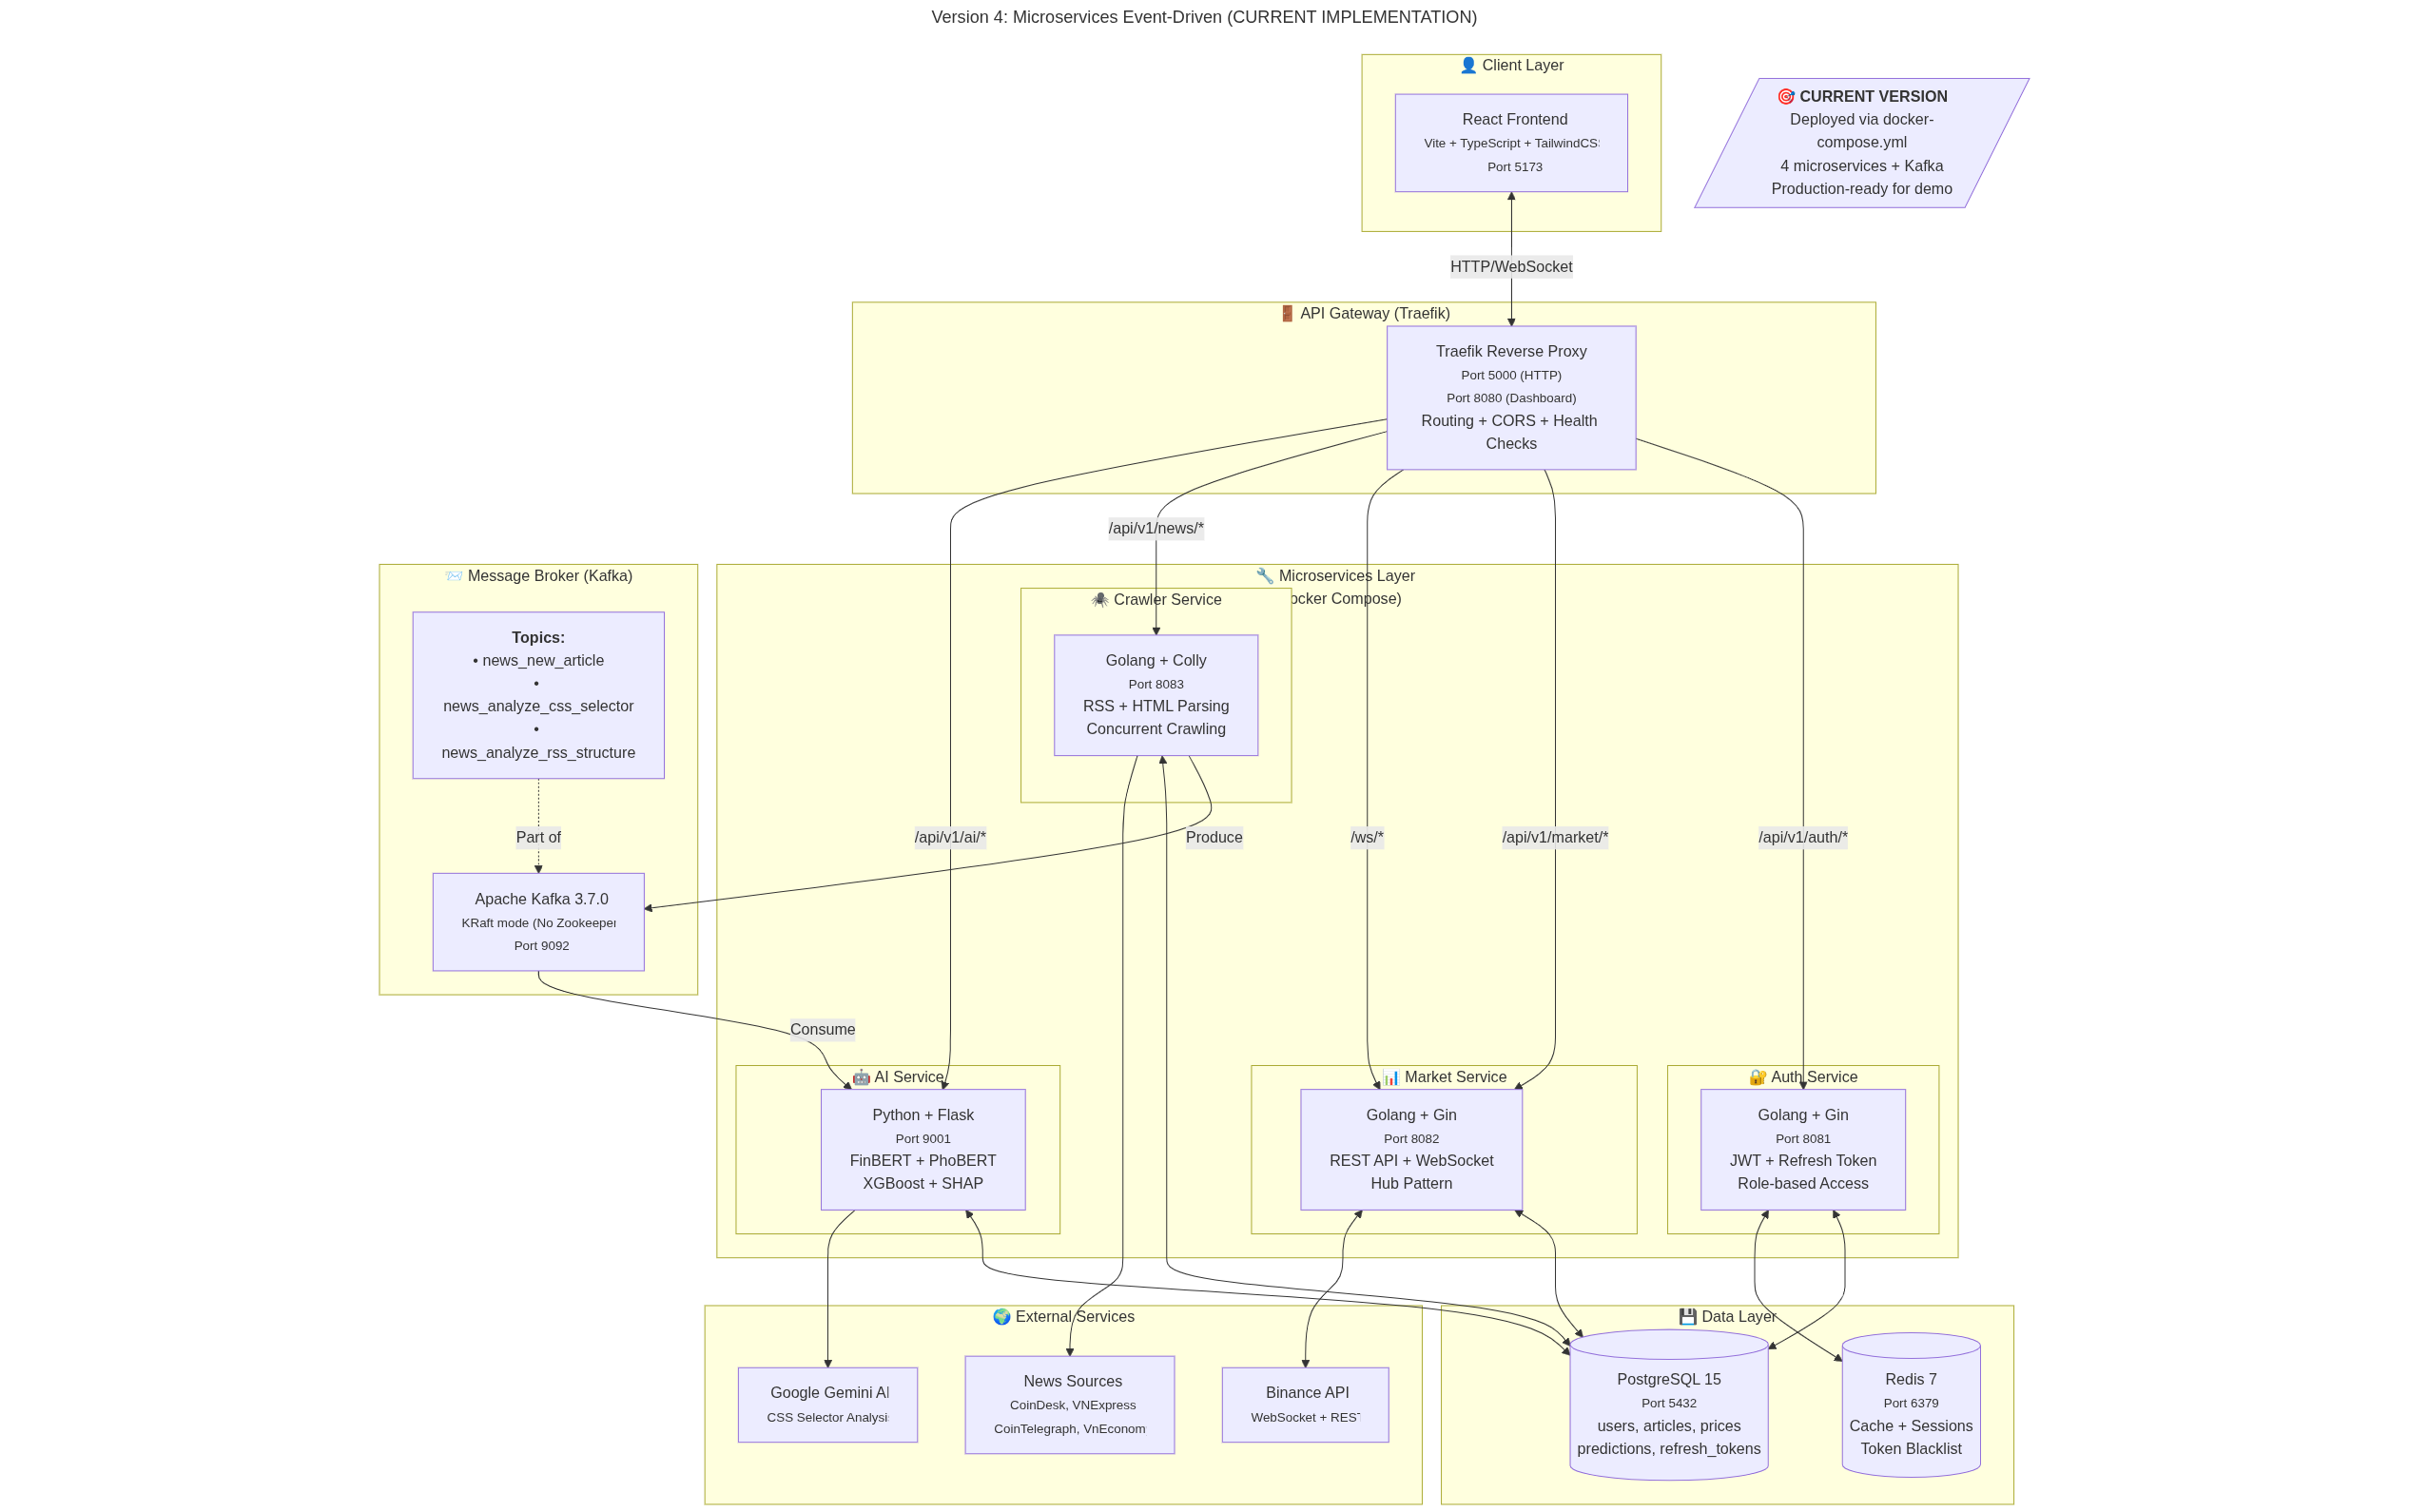
\includegraphics[width=\textwidth]{arch/ver4.png}
\caption{Kiến trúc tổng quan hệ thống (Version 4: Microservices với Kafka Event-Driven)}
\label{fig:arch-v4-overview}
\end{figure}

\subsection{Các thành phần chính và vai trò}

\subsubsection{Client (Frontend)}

\begin{itemize}
    \item \textbf{Công nghệ}: React + TypeScript, Vite; giao diện web responsive.
    \item \textbf{Vai trò}: Người dùng tương tác với hệ thống qua trình duyệt; gọi REST API để đăng nhập, lấy giá, tin tức, dự đoán AI; kết nối WebSocket để nhận dữ liệu giá realtime.
    \item \textbf{Lưu ý}: Client chỉ giao tiếp với API Gateway (HTTPS), không kết nối trực tiếp đến backend services.
\end{itemize}

\subsubsection{API Gateway (Traefik)}

\begin{itemize}
    \item \textbf{Vai trò}: Điểm vào duy nhất (single entry point) cho tất cả client requests; định tuyến theo path:
    \begin{itemize}
        \item \texttt{/api/v1/auth/*} $\to$ Auth Service (port 8081)
        \item \texttt{/api/v1/market/*} $\to$ Market Service (port 8082)
        \item \texttt{/ws/*} $\to$ Market Service WebSocket
        \item \texttt{/api/v1/news/*} $\to$ Crawler Service (port 8083)
        \item \texttt{/api/v1/ai/*} $\to$ AI Service (port 9001)
    \end{itemize}
    \item \textbf{Chức năng}: CORS handling, health checks, load balancing (khi scale nhiều instance), dashboard tại port 8080.
\end{itemize}

\subsubsection{Auth Service}

\begin{itemize}
    \item \textbf{Công nghệ}: Golang, Gin framework, GORM.
    \item \textbf{Vai trò}: Xác thực và phân quyền; đăng ký/đăng nhập với bcrypt; JWT Access Token (short-lived) + Refresh Token (long-lived, lưu DB); role-based access (NORMAL/VIP/ADMIN); token rotation và revoke.
\end{itemize}

\subsubsection{Market Service}

\begin{itemize}
    \item \textbf{Công nghệ}: Golang, WebSocket (gorilla/websocket).
    \item \textbf{Vai trò}: Kết nối Binance WebSocket API; nhận dữ liệu giá realtime; Hub pattern quản lý hàng nghìn client; topic-based subscription (theo symbol); lưu lịch sử giá vào PostgreSQL; publish updates lên Kafka.
\end{itemize}

\subsubsection{Crawler Service}

\begin{itemize}
    \item \textbf{Công nghệ}: Golang, Colly, gofeed.
    \item \textbf{Vai trò}: Thu thập tin tức từ RSS feeds (CoinDesk, CoinTelegraph, VNExpress); crawl HTML; produce Kafka messages (\texttt{news\_new\_article}, \texttt{news\_analyze\_css\_selector}) để AI Service xử lý.
\end{itemize}

\subsubsection{AI Service}

\begin{itemize}
    \item \textbf{Công nghệ}: Python, Flask, Transformers, XGBoost, SHAP.
    \item \textbf{Vai trò}: Consume Kafka từ Crawler; phân tích sentiment (FinBERT/PhoBERT); dự đoán giá (XGBoost + SHAP XAI); Gemini AI học CSS selectors.
\end{itemize}

\subsubsection{Message Broker (Apache Kafka)}

\begin{itemize}
    \item \textbf{Vai trò}: Giao tiếp bất đồng bộ giữa Crawler và AI; topics: \texttt{news\_new\_article}, \texttt{news\_analyze\_css\_selector}; cho phép replay, decoupling, và scale consumers độc lập.
\end{itemize}

\subsubsection{Database (PostgreSQL) và Cache (Redis)}

\begin{itemize}
    \item \textbf{PostgreSQL}: Cơ sở dữ liệu chính; bảng users, refresh\_tokens, sources, articles, market\_prices; shared cho các services trong implementation hiện tại.
    \item \textbf{Redis}: Cache giá hiện tại, top news; JWT blacklist; session/refresh token storage.
\end{itemize}

\subsection{Phân tích kiến trúc theo các tiêu chí}

\subsubsection{Hiệu năng (Performance)}

\begin{itemize}
    \item \textbf{WebSocket thay cho Polling}: Dữ liệu giá push-based, độ trễ thấp (hàng ms thay vì hàng giây).
    \item \textbf{Redis caching}: Giảm tải truy vấn DB cho hot data (giá, top news).
    \item \textbf{Event-driven}: Crawler và AI chạy async; AI chậm không block Crawler.
    \item \textbf{Phân tách domain}: Mỗi service tối ưu cho nhiệm vụ riêng (Golang cho I/O, Python cho AI).
\end{itemize}

\subsubsection{Khả năng mở rộng (Scalability)}

\begin{itemize}
    \item \textbf{Horizontal scaling}: Có thể scale từng service độc lập (vd. \texttt{docker-compose up -d --scale market-service=3}).
    \item \textbf{Topic-based WebSocket Hub}: Hỗ trợ nhiều client đồng thời; có thể mở rộng qua Kafka hoặc Redis Pub/Sub khi nhiều Market instances.
    \item \textbf{Kafka consumers}: Thêm consumer cho AI Service để tăng throughput xử lý tin tức.
\end{itemize}

\subsubsection{Độ tin cậy (Reliability)}

\begin{itemize}
    \item \textbf{Fault isolation}: AI Service crash không ảnh hưởng Market/Auth; Market Service vẫn phục vụ WebSocket khi Kafka tạm lỗi (graceful degradation).
    \item \textbf{Auto-reconnect}: Market Service kết nối lại Binance với exponential backoff khi mất kết nối.
    \item \textbf{Kafka replay}: Có thể replay messages nếu AI Service fail.
\end{itemize}

\subsubsection{Bảo mật (Security)}

\begin{itemize}
    \item \textbf{API Gateway}: Single entry point; kiểm tra CORS; có thể thêm rate limiting.
    \item \textbf{JWT + Refresh Token}: Access token ngắn hạn; Refresh token lưu DB, có thể revoke; rotation mỗi lần refresh.
    \item \textbf{Phân quyền}: Role-based (NORMAL/VIP/ADMIN); VIP required cho API AI.
    \item \textbf{Zero-Trust}: Mọi request phải authenticate; validate input; có thể mở rộng mTLS giữa services (Service Mesh).
\end{itemize}
